% !TEX root = ../dissertacao.tex
\acresetall{}
\chapter{Introdução}
\label{cap:introducao}


O paradigma de \ac{ood} surgiu no final da década de 80 e início dos anos 90.
Este paradigma teve como enfoque o aumento na produtividade de \textit{software} por meio da facilidade  no mapeamento dos objetos do mundo real para suas abstrações.
Este modelo é baseado em objetos, e não em dados e processamento como na programação estruturada.
Os objetos são organizados em classes de objetos e são associados a comportamentos.
Cada objeto é autocontido e possui todas as informações pertinentes para a realização das ações que ele representa~/~possui.
Este encapsulamento de informações facilita por sua vez a manutenção do código fonte e possibilita o desenvolvimento de \textit{software} em larga escala.


Embora o código orientado a objetos tenha seu lugar, ele tem sido a causa de muito tempo e esforço desperdiçados durante sua vida relativamente curta em nossa indústria de desenvolvimento de \textit{software} e desenvolvimento de jogos em particular~\cite{fabian2013data}.
O modelo \ac{ood} começa a mostrar suas fraquezas quando os projetos sofrem alterações.
% Estes projetos sofrem de uma inércia inerente ao manter o domínio do problema associado à implementação.
Quando os dados pertencentes ao \textit{software} sofrem algum tipo de alteração, muitas vezes é necessário que todo o \textit{software} seja reescrito para suportar estas alterações.
% Mantendo os dados separados das implementações que transformam estes dados, estas refatorações que seriam grandes e difíceis no modelo \ac{ood} tornam-se muitas vezes triviais~\cite{fabian2013data}.
Estas refatorações, que seriam grandes e difíceis no modelo \ac{ood}, tornam-se muitas vezes triviais quando os dados são isolados das implementações~\cite{fabian2013data}.

% problema na chamada de funções virtuais com OOD
% Outro problema enfrentado pela orientação a objetos é a iteração sobre um conjunto heterogêneo de objetos para a chamada de uma função virtual herdada de um outro objeto. A maneira padrão de iterar é através de um iterador e realizar a chamada da função virtual por meio deste iterador. Esta chamada implicará no carregamento do ponteiro da tabela virtual para cada objeto e irá causar uma espera pela carga do bloco da cache. Uma vez que o ponteiro da tabela virtual esteja carregado, ele poderá ser usado, com o deslocamento constante (o índice do método virtual), para encontrar o ponteiro de função a ser chamada (este deslocamento dependerá de cada objeto que estende o objeto pai portador da função virtual).

% vetorização de código:
Outro problema enfrentado pela orientação a objetos é a aplicação de uma mesma transformação (instrução) num grande conjunto de objetos.
Armazenando contiguamente os dados pertencentes ao mesmo domínio é possível aplicar esta transformação através de uma instrução \ac{simd}.
Já no modelo orientado a objetos faz-se necessário iterar sobre cada objeto e aplicar a transformação por meio de uma chamada de função pertencente a este objeto.
Uma forma de utilizar instruções \ac{simd} com orientação a objetos é armazenar os dados do mesmo domínio em uma estrutura contínua (como por exemplo um vetor) e cada objeto possuir uma referência para seu atributo nesta estrutura. Porém, este modelo traria complicações na manutenção adequada do objeto e pode vir a causar problemas no desenvolvimento, como por exemplo o acesso livremente a atributos que deveriam ser privativos de um objeto.

% transição de problemas em OOD para game engines e síntese física
Instruções \ac{simd} viabilizam que aplicações operem eficientemente sob um grande conjunto de dados.
Um exemplo destas aplicações são as \textit{Game engines} contemporâneas que devem renderizar gráficos 3D em imagens de altíssima resolução, modelar sistemas físicos realistas e também processar sistemas complexos de inteligência artificial num curto espaço de tempo.
Para atender a esses requisitos, vários conceitos e padrões de projetos são aplicados durante o desenvolvimento de um jogo para explorar as arquiteturas modernas de computadores, onde o acesso a memória representa o principal gargalo. 
Um dos conceitos empregados durante o desenvolvimento de \textit{game engines} é chamado de \ac{dod}. 
% Ao contrário do tradicional \ac{ood}, que se concentra em como os objetos modelam as entidades do problema, o \ac{dod} foca em como os dados serão organizados na memória.
% Esse modelo de programação pode reduzir a complexidade do \textit{software} e visa um processamento mais eficiente, explorando os recursos disponíveis do computador, como por exemplo os recursos de subsistema de memória e a capacidade de multiprocessamento.
Este modelo de programação foca em como os dados serão organizados na memória visando um processamento mais eficiente e explora os recursos disponíveis no computador, como por exemplo os recursos do subsistema de memória, a capacidade de multiprocessamento e a execução de instruções \ac{simd}.
Da mesma forma que as \textit{game engines}, as ferramentas de \ac{eda} devem ser capazes de lidar com um grande volume de dados com um curto tempo de execução.
Adicionalmente, o prazo entre o projeto e a fabricação de um chip é cada vez mais limitado para que um novo produto eletrônico possa garantir o mercado (\textit{time-to-market})~\cite{papa2011physical}.


O modelo \ac{ood} faz uso intensivo de herança entre as classes de objetos.
Esta herança tende a criar hierarquias de classes complexas, dificultando a manutenção do \textit{software}~\cite{nystrom2014game}. 
Embora o modelo \ac{dod} possa diminuir essas limitações, a modelagem das estruturas e relações complexas não são tão naturais quanto no modelo \ac{ood}.
Por este motivo, um padrão de projeto chamado \textit{Entity-Component System} é amplamente adotado no desenvolvimento de \textit{game engines} para lidar eficientemente com a criação e destruição de entidades, e também para gerenciar seus dados subjacentes (denominados de propriedades) \cite{wiebusch2015decoupling, zu2014campvis}.
Este sistema também pode substituir árvores de herança por relações simples, como agregação e composição, para construir um \textit{software} mais robusto e modular.

% problema de hierarquia de classes
Para ilustrar algumas dificuldades decorrentes do uso intensivo de herança proporcionado pelo modelo \ac{ood}, consideremos o desenvolvimento de uma biblioteca de \textit{software} para resolver problemas relacionados à síntese física (\textit{Physical Design}) de circuitos integrados seguindo a metodologia \textit{standard cells}\footnote{A metodologia \textit{standard cell} baseia-se na utilização de leiautes pré-projetados, referenciados por células, a serem usados na fabricação em silício das portas lógicas, flip-flops e outros elementos mais complexos. As informações geométricas (dimensões, posições dos pinos, bloqueios para roteamento etc) e as informações elétricas de cada célula (atraso, potência etc), necessárias para garantir o sucesso da síntese física, são reunidas em um repositório denominado de biblioteca de células ~\cite{kahng2011vlsi}.}.
% \footnote{A metodologia \textit{standard cell} é baseada na utilização de células pré-projetadas e tem como objetivo a redução do esforço do projeto. Tais células estão organizadas como uma biblioteca que reúne os leiautes pré-projetados de portas lógicas, flip-flops e eventualmente de elementos mais complexos, bem como diversas outras informações importantes para garantir o sucesso da síntese física do circuito: dimensões do leiaute, posição dos pinos, atraso, potência etc~\cite{kahng2011vlsi}.}.
Dentre tais problemas está a estimativa do comprimento de uma interconexão entre duas portas lógicas (células).
Neste contexto, considere a Figura~\ref{subfig:circuit_example}, a qual apresenta um exemplo do um circuito digital contendo duas portas lógicas (A e B), quatro interconexões (N1 a N4) e oito pinos (P1 a P8).

\begin{figure}[ht]
    \centering
    \subfigure[]{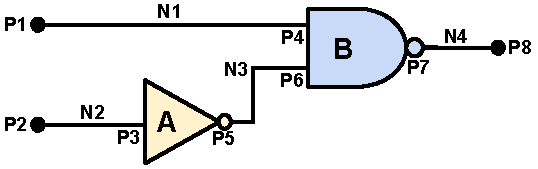
\includegraphics[width=0.6\linewidth]{img/introducao/circuitExample.pdf} \label{subfig:circuit_example}}
    
    \subfigure[]{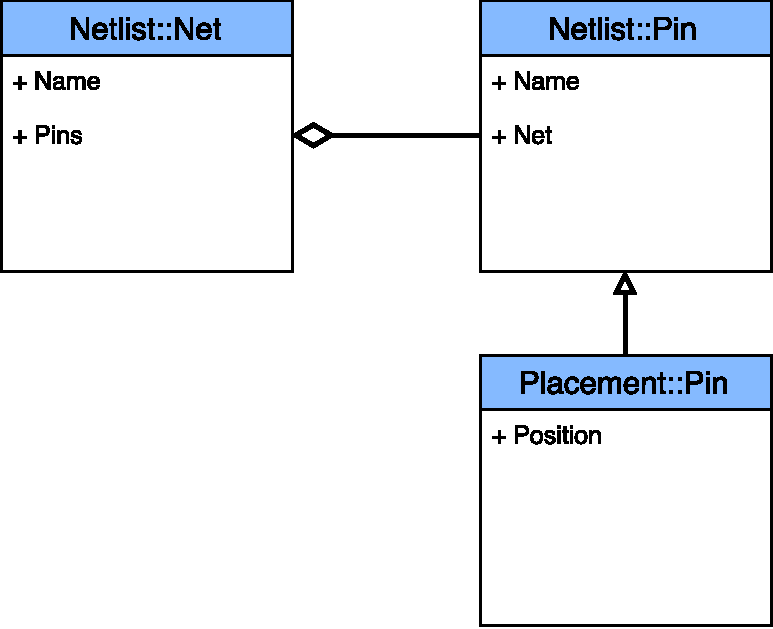
\includegraphics[width=0.38\linewidth]{img/introducao/classHierarchyOOD.pdf} \label{subfig:classHierarchyOOD}}
    \hspace{0.5cm}
    \subfigure[]{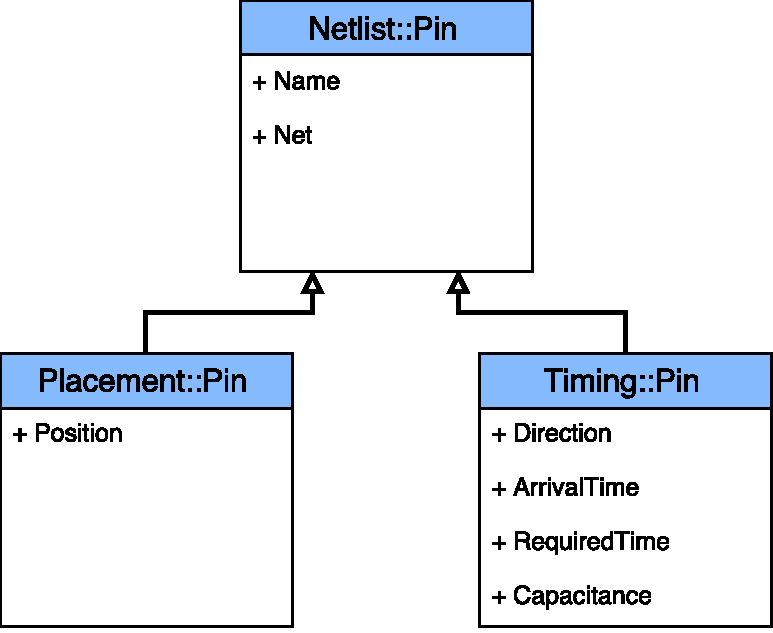
\includegraphics[width=0.38\linewidth]{img/introducao/classHierarchyTimingOOD.pdf} \label{subfig:classHierarchyTimingOOD}}
    \caption[Exemplo de um circuito digital]{Exemplo de um circuito digital (a) e dois possíveis diagramas de classe (b) (c) para o problema de estimar o comprimento de uma interconexão.}
    \label{fig:circuit_example}
\end{figure}

A Figura~\ref{subfig:classHierarchyOOD} apresenta o diagrama de classes para uma modelagem, segundo o modelo \ac{ood}, da estimativa do comprimento de interconexão que considera dois módulos: \textit{netlist} e \textit{placement}.
O módulo \textit{netlist} possui as classes \textit{net} e \textit{pin} para descrever as interconexões do circuito e os pinos associados, respectivamente.
Para a classe \textit{pin}, o módulo \textit{netlist} caracteriza apenas o nome do pino e a interconexão à qual esse pino pertence, sem nenhuma informação de posicionamento.
O módulo \textit{placement}, por sua vez, descreve as posições dos pinos.
A seta com ponta de losango entre as classes \textit{pin} e \textit{net} representa uma relação de agregação, o que significa que uma interconexão possui
referência aos seus pinos, enquanto um pino possui referência à interconexão à qual ele pertence. A seta de ponta triangular entre as duas classes \textit{pin} representa um relacionamento de hierarquia, o que significa que a classe \textit{pin} do módulo \textit{placement} estende os atributos da classe \textit{pin} no módulo \textit{netlist}.

Porém, quando as informações da temporização dos pinos forem necessárias, a classe \textit{pin} do módulo \textit{netlist} apresentada na Figura~\ref{subfig:classHierarchyOOD} deverá ser estendida 
por uma nova classe \textit{Pin} pertencente ao módulo \textit{Timing}, conforme mostrado na Figura~\ref{subfig:classHierarchyTimingOOD}.
Contudo, problemas que necessitem de informações de posicionamento e temporização (como por exemplo algoritmos de \ac{itdp}) deverão possuir informações de posicionamento e tempo.
Seguindo o modelo \ac{ood}, isso pode ser feito através de herança múltipla, onde uma nova classe \textit{pin} estende as classes \textit{pin} dos módulos \textit{placement} e \textit{timing}.
No entanto, a herança múltipla não é suportada por todas as linguagens de programação e, mesmo quando suportada, não é recomendada porque isso pode levar a problemas na modelagem do \textit{software}~\cite{nystrom2014game}.

\begin{figure}[h!b]
    \centering
    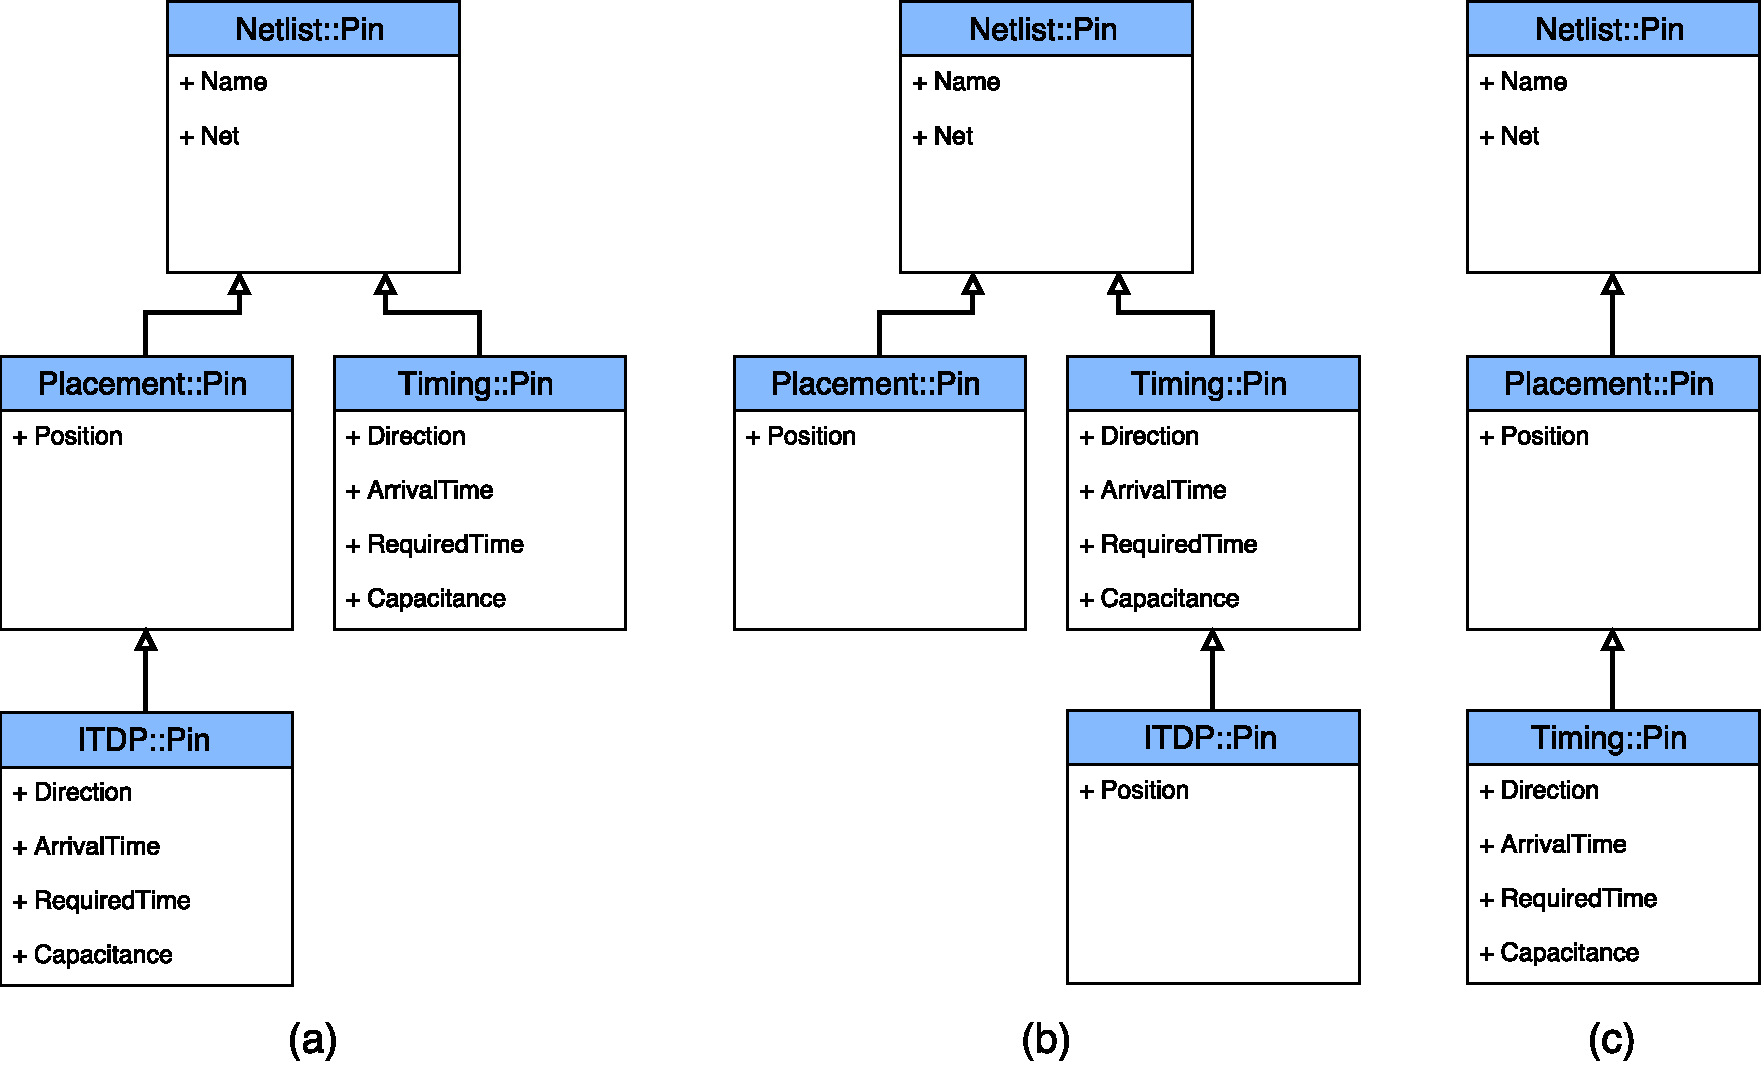
\includegraphics[width=0.8\textwidth]{img/introducao/ITDPsolutionOOD.pdf}
    % \caption{Class Hierarchy OOD.}
    \caption[Hierarquia de classes]{Possível hierarquia de classes para suportar informações de posicionamento e tempo para um algoritmo de \textit{timing-driven placement} utilizando o  modelo \ac{ood}.}
    \label{fig:classITDP}
\end{figure}

Sem recorrer à herança múltipla, a solução consiste em criar uma nova classe \textit{pin} que se estende a partir do módulo \textit{placement} ou \textit{timing} e possui repetição do código da outra classe (que não foi estendida). As Figuras~\ref{fig:classITDP} (a) e (b) mostram essas duas soluções. De qualquer forma, não há maneira simples de reutilizar informações de posicionamento e tempo sem ocorrer replicação de informações. A única opção que resta é juntar todas as informações na classe \textit{pin} do módulo \textit{timing} fazendo com que estenda a classe \textit{pin} do módulo \textit{placement}. Esta solução é ilustrada na Figura~\ref{fig:classITDP} (c). No entanto, nem sempre é necessário ter informações de posicionamento no módulo \textit{timing}. Por exemplo, uma ferramenta de \ac{sta} pode não precisar de informações de posicionamento durante as primeiras etapas de projeto. Portanto, a adoção da última solução levaria ao desperdício da localidade espacial da memória \textit{cache}, já que informações desnecessárias seriam recuperadas juntamente com informações úteis.





% Da mesma forma que as \textit{game engines}, as ferramentas de \ac{eda} devem ser capazes de lidar com um grande volume de dados com um curto tempo de execução.
% Adicionalmente, o prazo entre o projeto e a fabricação de um chip é cada vez mais limitado para que um novo produto eletrônico possa garantir o mercado (\textit{time-to-market})~\cite{papa2011physical}.
% Para isso, estas ferramentas devem empregar otimizações de \textit{software}, como o uso de melhores organizações nos dados, estruturas de dados otimizadas, paralelização e exploração da localidade de dados na \textit{cache}.
Para garantir tempos de execução aceitáveis, as ferramentas de \ac{eda} devem explorar ao máximo as otimizações de \textit{software}, como por exemplo: o uso de estruturas de dados otimizadas, paralelização e exploração da localidade da memória \textit{cache}.
Se examinarmos as ferramentas atuais de \ac{eda} disponibilizadas pela academia, como por exemplo aquelas descritas por \citeonline{universityOfMichigan, kahng2014horizontal, jung2016opendesign, flach2017rsyn, openAccess}, todas elas realizam uma série de otimizações de \textit{software}, mas nenhuma se concentra na organização de dados para explorar a localidade espacial da memória \textit{cache}.
Já os trabalhos que focam na exploração da localidade espacial e temporal dos dados, como os de \citeonline{li2014, Tang2015, qasem2017characterizing}, não realizam avaliações no contexto da síntese física.
O presente trabalho se concentra na discussão e aplicação desses conceitos modernos de engenharia de \textit{software} no desenvolvimento de ferramentas para a síntese física de \acp{ic}.

\section{Justificativa}

    Apesar de vários trabalhos encontrados na literatura fizeram otimizações de \textit{software} mencionadas na seção anterior, nenhum deles avalia o impacto destas diferentes estratégias quando aplicadas no contexto da síntese física.

    % Portanto, é desejável uma análise quantitativa do impacto da organização dos dados no contexto de Physical Design, sobretudo, com uma comparação que faça uso de uma infraestrutura realista e bem consolidada na academia.
    Portanto, é desejável uma análise quantitativa do impacto da organização dos dados no contexto da síntese física, sobretudo, com um estudo de problemas reais utilizando entradas realistas para a experimentação.

\section{Objetivos e Contribuições Alcançadas}

    % Este trabalho tem como objetivo a avaliação quantitativa do impacto causado pela organização dos dados em diferentes algoritmos utilizados na síntese física, que possuam diferentes características.
    Este trabalho possui como objetivo a avaliação quantitativa do impacto da organização dos dados em algoritmos de síntese física. 
    A fim de tentar permitir uma extrapolação das conclusões de tal avaliação para algoritmos semelhantes em outros domínios de aplicação, este trabalho também sistematiza as principais características e estruturas de dados dos algoritmos aqui avaliados.
    % Para isso, a fim de garantir uma ampla completude das características da síntese física, são elencadas as principais características e estruturas de dados destes algoritmos.

    Os objetivos específicos deste trabalho são:

    \begin{itemize}
        % \item Implementar um conjunto de algoritmos da síntese física que possuam diferentes características;
        \item Avaliar as organizações de dados propostas, comparando-as com a modelagem baseada em orientação a objetos. A comparação é realizada avaliando-se o número de \textit{cache misses} gerados pelas implementações dos algoritmos, bem como os tempos de execução associados;
        \item Investigar possíveis otimizações na organização dos dados para cada algoritmo implementado;
        \item Avaliar o desempenho da paralelização dos algoritmos implementados com as diferentes organização dos dados.
    \end{itemize}

\section{Contribuições científicas e tecnológicas}

    Este trabalho traz as seguintes contribuições científicas e tecnológicas:

    \begin{itemize}
        \item Implementação de um sistema de componentes e entidades. Estes conceitos serão detalhados na Seção~\ref{sec:entity_component_system};
        \item Avaliação quantitativa do desempenho resultante da modelagem dos dados em algoritmos utilizados na síntese física;
        \item Resultados experimentais utilizando casos de uso realistas. Como dados de entrada são utilizados circuitos industriais oriundos da competição ICCAD CAD Context 2015~\cite{kim2015};
        \item Comparação quantitativa do número de \textit{cache misses} e do tempo de execução para quatro algoritmos da síntese física.  
    \end{itemize}


% \section{Metodologia}
%         Implementar versões de problemas
%         avaliar quantitativamente o número de cache misses
%         avaliar quantitativamente o tempo de execução
%
% \section{Limitações(escopo) deste trabalho}
%         somente 3 problemas avaliados
%         somente uma arquitetura de processador e cache
%         paralelização com um chunk único

% \section{Organização deste trabalho}
\section{Organização deste trabalho}

O Capítulo~\ref{cap:conceitos_fundamentais} revisa alguns conceitos fundamentais para a melhor compreensão deste trabalho.
No Capítulo~\ref{cap:trabalhos_correlatos} são apresentados os trabalhos correlatos na otimização da organização dos dados para uma melhor utilização da memória \textit{cache}.
O Capítulo~\ref{cap:tecnica_proposta} descreve a proposta de organização dos dados e seus possíveis impactos no contexto da síntese física.
O Capítulo~\ref{cap:caracterizacaoSinteseFisica} apresenta, de forma sintética, as etapa pertencentes à síntese e caracteriza os algoritmos envolvidos em cada etapa.
No Capítulo~\ref{cap:resultados} são apresentadas as organizações dos dados utilizadas em cada estudo de caso e os respectivos resultados experimentais.
Por fim, o Capítulo~\ref{cap:conclusao_e_trabalhos_futuros} apresenta as conclusões obtidas com a realização deste trabalho e os possíveis desdobramentos futuros.

